%% Pipeline overview (Figure 1 of the article). Compiled to figures/pipeline.pdf
%% and figures/pipeline.png by tools/make_pipeline_figure.py. It is a schematic,
%% not a data figure: every quantity it names is stated in the article's text.
%% Fonts match the manuscript (cas-dc loads STIX and Inconsolata); colours are
%% from the Okabe-Ito palette used by the data figures. The drawing is sized to
%% the cas-dc text width (494.5pt), so it is included at its natural size.
\documentclass[tikz,border=1pt]{standalone}
\usepackage[T1]{fontenc}
\usepackage{stix}
\usepackage[scaled=.85]{inconsolata}
\usetikzlibrary{positioning,arrows.meta,fit,backgrounds,calc}

\definecolor{okblue}{HTML}{0072B2}
\definecolor{okverm}{HTML}{D55E00}
\definecolor{okgreen}{HTML}{009E73}

\newcommand{\id}[1]{\texttt{#1}}
\newcommand{\head}[1]{{\footnotesize\bfseries #1}\\[1.5pt]}

\begin{document}
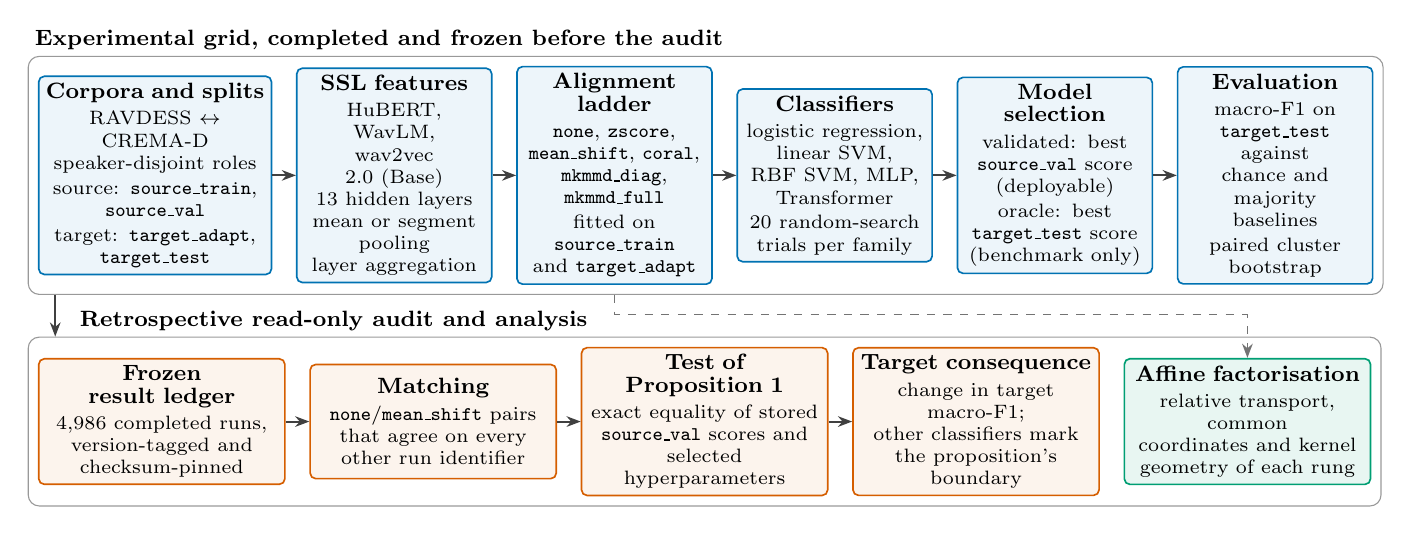
\begin{tikzpicture}[
  font=\scriptsize,
  node distance=0.3cm,
  box/.style={line width=0.6pt, rounded corners=2pt, align=center,
    inner sep=2.5pt,
    execute at begin node={\hyphenpenalty=10000\exhyphenpenalty=10000}},
  stage/.style={box, draw=okblue, fill=okblue!7, text width=2.3cm,
    minimum height=2.05cm},
  wide/.style={stage, text width=2.78cm},
  audit/.style={box, draw=okverm, fill=okverm!7, text width=2.95cm,
    minimum height=1.45cm},
  theory/.style={box, draw=okgreen, fill=okgreen!9, text width=2.95cm,
    minimum height=1.45cm},
  flow/.style={-{Stealth[length=1.8mm]}, line width=0.7pt, draw=black!75},
  side/.style={-{Stealth[length=1.8mm]}, line width=0.6pt, draw=black!55,
    dashed},
  lane/.style={draw=black!40, rounded corners=4pt, inner sep=3.5pt},
  lanetitle/.style={font=\footnotesize\bfseries, anchor=south west,
    inner sep=1pt},
]

% ---- top lane: the experimental grid ------------------------------------
\node[wide] (corp) {\head{Corpora and splits}
  RAVDESS $\leftrightarrow$ CREMA-D\\ speaker-disjoint roles\\[1pt]
  source: \id{source\_train},\\ \id{source\_val}\\[1pt]
  target: \id{target\_adapt},\\ \id{target\_test}};
\node[stage, right=of corp] (feat) {\head{SSL features}
  HuBERT, WavLM,\\ wav2vec 2.0 (Base)\\ 13 hidden layers\\
  mean or segment\\ pooling\\ layer aggregation};
\node[stage, right=of feat] (align) {\head{Alignment ladder}
  \id{none}, \id{zscore},\\ \id{mean\_shift}, \id{coral},\\
  \id{mkmmd\_diag}, \id{mkmmd\_full}\\[1pt] fitted on \id{source\_train}\\
  and \id{target\_adapt}};
\node[stage, right=of align] (clf) {\head{Classifiers}
  logistic regression,\\ linear SVM,\\ RBF SVM, MLP,\\ Transformer\\[1pt]
  20 random-search\\ trials per family};
\node[stage, right=of clf] (sel) {\head{Model selection}
  validated: best\\ \id{source\_val} score\\ (deployable)\\[1pt]
  oracle: best\\ \id{target\_test} score\\ (benchmark only)};
\node[stage, right=of sel] (eval) {\head{Evaluation}
  macro-F1 on\\ \id{target\_test} against\\ chance and majority\\
  baselines\\[1pt] paired cluster\\ bootstrap};

\foreach \a/\b in {corp/feat, feat/align, align/clf, clf/sel, sel/eval}
  \draw[flow] (\a) -- (\b);

% ---- bottom lane: the retrospective audit -------------------------------
\node[audit, below=1.05cm of corp.south west, anchor=north west] (ledger)
  {\head{Frozen result ledger}
  4,986 completed runs,\\ version-tagged and\\ checksum-pinned};
\node[audit, right=of ledger] (match) {\head{Matching}
  \id{none}/\id{mean\_shift} pairs\\ that agree on every\\
  other run identifier};
\node[audit, right=of match] (prop) {\head{Test of Proposition~1}
  exact equality of stored\\ \id{source\_val} scores and\\
  selected hyperparameters};
\node[audit, right=of prop] (out) {\head{Target consequence}
  change in target macro-F1;\\ other classifiers mark\\
  the proposition's boundary};
\node[theory, right=of out] (fact) {\head{Affine factorisation}
  relative transport, common\\ coordinates and kernel\\
  geometry of each rung};

\foreach \a/\b in {ledger/match, match/prop, prop/out}
  \draw[flow] (\a) -- (\b);

% ---- lane frames and titles ----------------------------------------------
\begin{scope}[on background layer]
  \node[lane, fit=(corp)(eval)] (gridlane) {};
  \node[lane, fit=(ledger)(match)(prop)(out)(fact)] (auditlane) {};
\end{scope}
\node[lanetitle] at ($(gridlane.north west)+(0.05,0.03)$)
  {Experimental grid, completed and frozen before the audit};
% The bottom title starts to the right of the inter-lane arrow so that the
% arrow never crosses it.
\node[lanetitle] at ($(auditlane.north west)+(0.62,0.03)$)
  {Retrospective read-only audit and analysis};

% Every run of the grid is recorded in the ledger; the factorisation analyses
% the maps of the alignment ladder.
\draw[flow] ($(gridlane.south west)+(0.35,0)$)
  -- ($(auditlane.north west)+(0.35,0)$);
\draw[side] (align.south |- gridlane.south)
  -- ++(0,-0.25) -| (fact.north);

\end{tikzpicture}
\end{document}
